\scanpage{40}
\mspage{21}
Je vais expliciter les calculs $\underset{\unsure{\wedge}}{\vphantom{x}}$ dans le groupoïde $\overline{\underline{\mathrm{VII}}}$, associé au graphe de $=$ nom, on a des flèches génératrices
\[
(71)\qquad\left\{\begin{aligned}
\widetilde d_i^\omega&:P^\omega\mathpunct{.}\longrightarrow R_i^\omega\\
\widetilde d_i^{\prime\omega}&:P^\omega\longrightarrow R_i^{\omega'}\\
a_i^\omega&:R_i^\omega\mathbin{-}R_i^{\omega'}
\end{aligned}\right.
\]
liées par les relations
\[
(72)\qquad\left\{\begin{aligned}
(\widetilde d_i^{\prime\omega})^{-1}a_i^\omega\widetilde d_i^\omega&=1\\
(d_{\omega i}^{\prime\omega})^{-1}d_{\omega i}^{\omega'}(d_i^{\prime\omega'})^{-1}d_i^\omega&=1
\end{aligned}\right.
\]
\margin{six relations indépendantes exprimant les $\widetilde d_i^{\prime\omega}$ en termes des $\widetilde d_i^\omega$ et $a_i^\omega$, \inserted{ou les $\unsure{a_i^\omega}$ en termes des $\widetilde d_i^\omega,\unsure{\widetilde d_i^{\prime\omega}|d_i^{\prime\omega}}$.}}
\margin{en apparence six relations, mais il n'y en a que trois indépendantes, car l'équation pour $i,\omega$ et pour $(\omega i,\omega')$ est la $=$.}
\figure{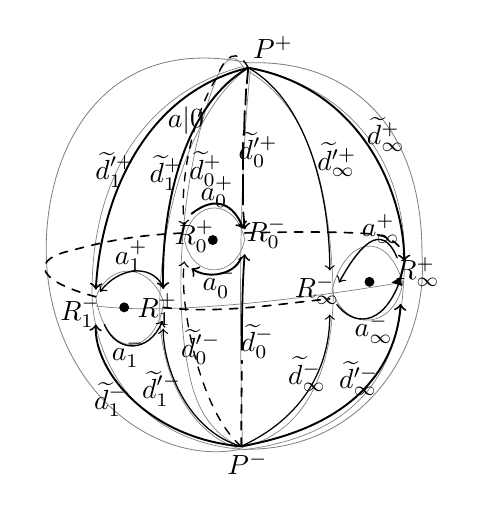
\begin{tikzpicture}[x=.009cm,y=-.009cm,line cap=round,line join=round]
\coordinate (P) at (360,1172);
\coordinate (M) at (350,1706);
\draw[gray,line width=.3pt] (360,1165)..controls (140,1120) and (65,1310)..(76,1455)..controls (90,1630) and (230,1735)..(350,1710)..controls (520,1715) and (615,1570)..(605,1435)..controls (606,1250) and (500,1160)..(360,1165);
\draw[gray,line width=.25pt] (353,1170)..controls (185,1215) and (135,1370)..(140,1503)..controls (151,1620) and (230,1700)..(348,1710);
\draw[gray,line width=.25pt] (357,1174)..controls (273,1240) and (236,1390)..(235,1510)..controls (235,1620) and (290,1695)..(350,1710);
\draw[gray,line width=.25pt] (354,1174)..controls (343,1150) and (329,1155)..(316,1185)..controls (270,1300) and (251,1480)..(276,1600)..controls (288,1664) and (317,1692)..(349,1707);
\draw[gray,line width=.25pt] (363,1176)..controls (347,1320) and (347,1530)..(352,1708);
\draw[gray,line width=.25pt] (360,1177)..controls (456,1233) and (476,1365)..(480,1492)..controls (478,1615) and (430,1690)..(352,1707);
\draw[gray,line width=.25pt] (365,1172)..controls (535,1210) and (591,1340)..(579,1475)..controls (573,1610) and (505,1692)..(352,1711);
\draw[gray,line width=.25pt] (145,1496)..controls (165,1443) and (222,1448)..(241,1503)..controls (228,1582) and (160,1585)..(145,1496);
\draw[gray,line width=.25pt] (270,1414)..controls (282,1355) and (342,1355)..(355,1414)..controls (344,1470) and (281,1473)..(270,1414);
\draw[gray,line width=.25pt] (478,1486)..controls (497,1412) and (554,1398)..(578,1475)..controls (568,1539) and (499,1548)..(478,1486);
\draw[gray,line width=.25pt] (145,1508)..controls (246,1521) and (428,1500)..(575,1475);
\draw[dashed,line width=.6pt] (145,1495)..controls (50,1470) and (60,1440)..(110,1430)..controls (180,1410) and (230,1407)..(270,1405);
\draw[dashed,line width=.6pt] (355,1405)..controls (424,1403) and (499,1403)..(540,1407)..controls (564,1412) and (576,1423)..(581,1440);
\draw[dashed,line width=.6pt] (240,1510)..controls (320,1520) and (410,1504)..(475,1498);
\fill (185,1510) circle[radius=7];
\fill (310,1415) circle[radius=7];
\fill (531,1474) circle[radius=7];
\draw[->,line width=.7pt] (P)..controls (205,1210) and (151,1370)..(145,1485);
\draw[->,line width=.7pt] (P)..controls (260,1230) and (237,1390)..(240,1484);
\draw[dashed,->,line width=.5pt] (P)..controls (345,1143) and (327,1154)..(316,1185)..controls (278,1245) and (263,1340)..(270,1395);
\draw[line width=.65pt] (P)--(358,1194);
\draw[line width=.65pt] (357,1202)--(356,1224);
\draw[line width=.65pt] (355,1233)--(354,1267);
\draw[line width=.65pt] (353,1278)--(353,1315);
\draw[line width=.65pt] (353,1323)--(353,1365);
\draw[->,line width=.65pt] (353,1376)--(355,1400);
\draw[->,line width=.45pt] (P)..controls (445,1220) and (475,1355)..(475,1458);
\draw[->,line width=.7pt] (P)..controls (520,1200) and (580,1350)..(580,1445);
\draw[->,line width=.7pt] (M)..controls (220,1695) and (142,1600)..(145,1534);
\draw[->,line width=.45pt] (M)..controls (275,1685) and (240,1595)..(240,1540);
\draw[dashed,->,line width=.5pt] (M)..controls (290,1655) and (262,1500)..(270,1445);
\draw[dashed,line width=.65pt] (M)..controls (350,1660) and (351,1615)..(351,1585);
\draw[->,line width=.65pt] (351,1570)..controls (351,1520) and (352,1470)..(355,1435);
\draw[->,line width=.45pt] (M)..controls (450,1660) and (475,1580)..(475,1520);
\draw[->,line width=.7pt] (M)..controls (525,1675) and (570,1580)..(575,1505);
\draw[->,line width=.5pt] (239,1479)..controls (221,1447) and (176,1455)..(151,1488);
\draw[->,line width=.5pt] (157,1534)..controls (174,1575) and (220,1575)..(239,1529);
\draw[->,line width=.7pt] (280,1378)..controls (315,1350) and (340,1366)..(353,1399);
\draw[->,line width=.7pt] (350,1440)..controls (340,1465) and (302,1470)..(280,1455);
\draw[->,line width=.5pt] (570,1440)..controls (548,1387) and (516,1424)..(488,1475);
\draw[line width=.5pt] (485,1506)..controls (507,1535) and (548,1540)..(573,1475);
\fill (562,1475)--(575,1467)--(577,1480)--cycle;
\node at (395,1144) {$P^+$};
\node at (359,1730) {$P^-$};
\node at (272,1246) {$\unsure{a|0}$};
\node at (123,1517) {$R_1^-$};
\node at (232,1513) {$R_1^+$};
\node at (284,1410) {$R_0^+$};
\node at (386,1405) {$R_0^-$};
\node at (457,1485) {$R_\infty^-$};
\node at (599,1460) {$R_\infty^+$};
\node at (195,1438) {$a_1^+$};
\node at (191,1573) {$a_1^-$};
\node at (316,1347) {$a_0^+$};
\node at (319,1475) {$a_0^-$};
\node at (547,1399) {$a_\infty^+$};
\node at (537,1540) {$a_\infty^-$};
\node at (172,1316) {$\widetilde d_1^{\prime+}$};
\node at (244,1320) {$\widetilde d_1^+$};
\node at (300,1315) {$\widetilde d_0^+$};
\node at (374,1288) {$\widetilde d_0^{\prime+}$};
\node at (485,1302) {$\widetilde d_\infty^{\prime+}$};
\node at (554,1266) {$\widetilde d_\infty^+$};
\node at (166,1640) {$\widetilde d_1^-$};
\node at (238,1625) {$\widetilde d_1^{\prime-}$};
\node at (293,1566) {$\widetilde d_0^{\prime-}$};
\node at (373,1558) {$\widetilde d_0^-$};
\node at (443,1604) {$\widetilde d_\infty^-$};
\node at (516,1610) {$\widetilde d_\infty^{\prime-}$};
\end{tikzpicture}}
On va repérer $u$ par les équations
\[
(\unsure{73})\qquad\left\{\begin{aligned}
u(\widetilde d_i^\omega)&=\deleted{\unsure{\widetilde d_i^\omega}}\varphi_i^\omega(\xi_1^{\deleted{\unsure{1|'}}})\widetilde d_i^\omega\\
u(\widetilde d_i^{\prime\omega})&=\deleted{\unsure{\widetilde d_i^{\prime\omega}}}\varphi_i^{\omega'}(\xi')\widetilde d_i^{\prime\omega}\\
u(a_i^\omega)&=a_i^\omega\varphi_i^\omega(\lambda)
\end{aligned}\right.\qquad \xi',\xi_1^{\deleted{\unsure{'}}},\lambda\in\widehat\Pi_{03}
\]
et il reste à exprimer que $u$ satisfait les relations (72). La première s'explicite sous la forme
\[
(74)\qquad\xi'=\varepsilon_0(\lambda\xi_1)\qquad\text{i.e.}\quad\xi_1=\lambda^{-1}\cdot\varepsilon_0^{-1}(\xi')
\]
et on trouve également
\[
(75)\qquad\unsure{\deleted{\beta}|\beta}\xi_1=\beta'\sigma_\infty(\xi')
\]
\margin{où $\beta'$ défini par la condition $(65\,\unsure{a|'}))$}
Cette relations permettant de tirer $\beta'$ en termes
\margin{39}
